\chapter{Kravspecifikation}

%Moscow
Kravene til produktet er prioriteret ved brug af MoSCoW metoden. Her er kravene for produktet inddelt i fire kategorier, hvor de vigtigste elementer er prioriteret højest. \textbf{Must} benævner de krav som er vigtigst at opfylde, og som er absolut nødvendigt for produktet. \textbf{Should} er de krav produktet bør opfylde. \textbf{Could} er kravene som produktet evt. kunne opfylde, hvis projektets tidsramme tillader det. \textbf{Won't} er krav som ikke vil blive opfyldt inden for projektets tidsrammer, men evt. kan tages med i senere iterationer.

\noindent Følgende opdeling viser kravene udvalgt for dette projekt:
\begin{itemize}
	\item[\textbf{Must}]
		\begin{itemize}
			\item Have et funktionsdygtigt power-modul
			\item Ikke påvirke andre moduler ved fejl
			\item Have et termisk design, kompatibelt med vakuum
			\item Underbygges med en P-Spice model

		\end{itemize}
	\item[\textbf{Should}]
		\begin{itemize}
			\item Have programmerbar udgangsstrøm og -spænding
			\item Have stabil regulering
			\item Have overstrømsbeskyttelse på udgangen
			\item Have overspændingsbeskyttelse på udgangen

		\end{itemize}
	\item[\textbf{Could}] 
		\begin{itemize}
			\item Have mulighed for brug til mere end to forskellige typer loads
			\item Konstrueres med EEE komponenter

		\end{itemize}
	\item[\textbf{Won't}]
		\begin{itemize}
			\item Have feedback til brugeren når valgt load er aktiveret
			\item Have galvanisk adskillelse
			
		\end{itemize}
\end{itemize}

\clearpage



\section{Aktør diagrammer}
I det følgende afsnit illustreres systemets aktører i et aktør-kontekst diagram. Derudover gives et mere beskrivende indblik i aktørernes interaktion med systemets use cases, i et use case diagram.
\begin{figure}[H]
	\centering
	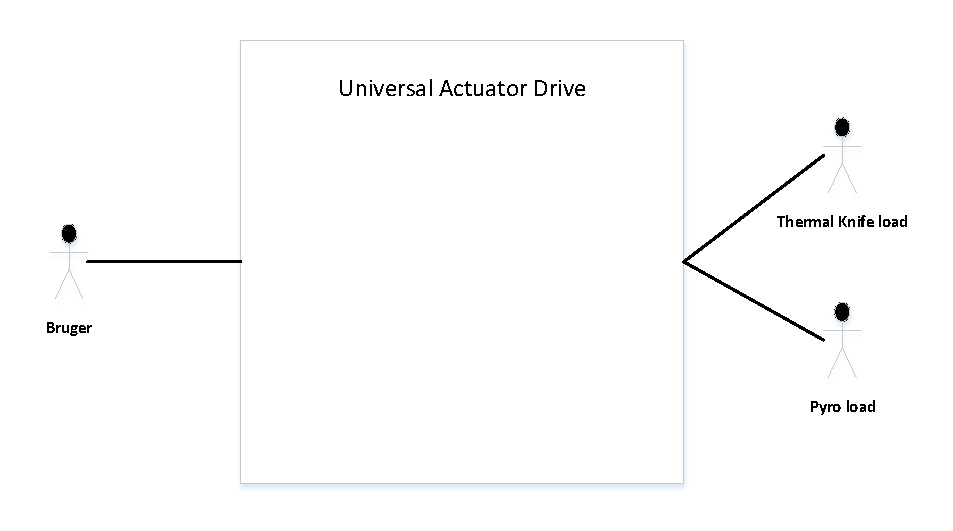
\includegraphics{tex/Kravspecifikation/billeder/AktorkontekstdiagramV1.pdf}
	\caption{Aktør-kontekst diagram}
\end{figure}

\begin{figure}[H]
	\centering
	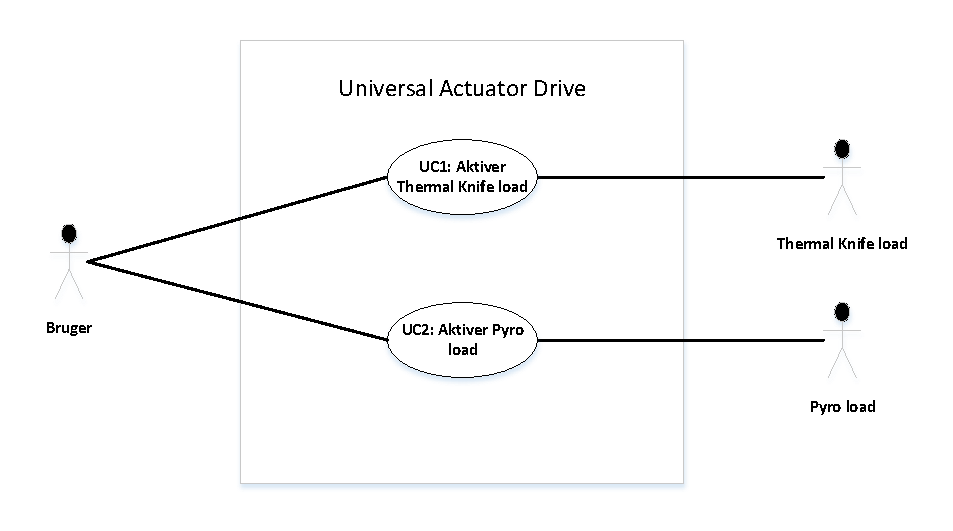
\includegraphics{tex/Kravspecifikation/billeder/UseCasediagramV1.pdf}
	\caption{Use case diagram}
\end{figure}




\section{Aktørbeskrivelse}
I det følgende afsnit beskrives systemets aktører. Ved hver aktør angives typen, samt en kort beskrivelse af aktørens funktion og/eller hvordan de påvirker systemet.

\begin{framed}
	\subsection{Aktør: Bruger}
	\subsubsection*{Type:}
		Primær
	
	\subsubsection*{Beskrivelse:}
		Brugeren interagerer med systemet, ved at indstille den ønskede load type.
\end{framed}

\begin{framed}
	\subsection{Aktør: Thermal Knife load}
	\subsubsection*{Type:}
	Sekundær
	
	\subsubsection*{Beskrivelse:}
	Thermal Knife load er en load type, hvor et varmelegeme opvarmes langsomt. \indent Denne type bruges til at skære reb over, og derved udløse diverse bevægelige \indent dele.
\end{framed}

\begin{framed}
	\subsection{Aktør: Pyro load}
	\subsubsection*{Type:}
	Sekundær
	
	\subsubsection*{Beskrivelse:}
	Pyro load er en load type, hvor en glødetråd opvarmes hurtigt. Denne type bru- \indent ges til at detonere en krudtladning, og derved sprænge en bolt, som frigør diverse \indent bevægelige dele.
\end{framed}

\clearpage

	

% Skabelon
%\begin{framed}
%\subsubsection{Mål:}
%
%\subsubsection{Initiering:}
%
%\subsubsection{Aktører:}
%
%\subsubsection{Referencer:}
%
%\subsubsection{Samtidige forekomster:}
%
%\subsubsection{Forudsætning:}
%
%\subsubsection{Resultat:}
%
%\subsubsection{Hovedscenarie:}
%
%\subsubsection{Extension:}

\section{Fully dressed use cases}

\begin{framed}
	\subsection{Use case 1 - Aktiver Thermal Knife load}
	\subsubsection*{Mål:}
	At aktivere Thermal Knife load
	
	\subsubsection*{Initiering:}
	Brugeren
	
	\subsubsection*{Aktører:}
	Brugeren (Primær)\\ \indent
	Thermal Knife load (Sekundær)
	
	\subsubsection*{Referencer:}
	Ingen
	
	\subsubsection*{Samtidige forekomster:}
	En
	
	\subsubsection*{Forudsætning:}
	Hverken Use case 1 eller Use case 2 er under udførelse
	
	
	\subsubsection*{Resultat:}
	Thermal knife load er aktiveret
	
	
	\subsubsection*{Hovedscenarie:}
	\begin{enumerate}
		\item Brugeren vælger Thermal knife load
		\item Systemet indstiller strøm og spænding til Pyro load
		\item Systemet aktiverer Thermal knife load
	\end{enumerate}
	
\end{framed}

\clearpage

\begin{framed}
	\subsection{Use case 2 - Aktiver Pyro load}
	
	\subsubsection*{Mål:}
	Aktiver Pyro load
	
	\subsubsection*{Initiering:}
	Bruger
	
	\subsubsection*{Aktører:}
	Bruger (Primær)\\ \indent
	Pyro load (Sekundær)
	
	\subsubsection*{Referencer:}
	Ingen
	
	\subsubsection*{Samtidige forekomster:}
	En
	
	\subsubsection*{Forudsætning:}
	Hverken Use case 1 eller Use case 2 er under udførelse
	
	\subsubsection*{Resultat:}
	Pyro load er aktiveret
	
	\subsubsection*{Hovedscenarie:}
	\begin{enumerate}
		\item Brugeren vælger Pyro load
		\item Systemet indstiller strøm og spænding til Pyro load %TODO Sammenhæng accepttest
		\item Systemet aktiverer Pyro load
	\end{enumerate}

\end{framed}

\clearpage

\section{Ikke-funktionelle krav}
I dette afsnit beskrives de ikke-funktionelle krav. Her opstilles f.eks. krav om præcision, brugervenlighed samt produktets dimensioner.
\begin{itemize}
			\item Inputspændingen skal være mellem 26-100V
			\item Der må maksimalt trækkes en peak-strøm fra inputkilden på 150\% af inputstrømmen
			\item Skal opretholde en outputspænding på op til 21V, $\pm$2\% ved 2,5A $\pm$5\%
			\item Skal opretholde en outputstrøm op til 5A $\pm$5\%, ved 15V $\pm$2\%
			\item Der må maksimalt være en ripple-spænding på 50mV pk-pk
			\item Der må maksimalt være switching spikes på 100mV pk-pk
			\item Skal kunne omsætte op til 75W
			\item Skal operere med et tab på maksimalt 5W %TODO Specificer tab nærmere
			\item Skal implementeres i et volumen mindre end 17x75x100mm på forsiden af PCB'et, samt 3x75x100mm på bagsiden af PCB'et
			\item Skal kunne operere med en omgivelsestemperatur mellem -35\degreeCelsius\  og 65\degreeCelsius\
			\item Skal have stabil regulering med 10dB gain og 50 graders fasemargin ved:
				\begin{description}
					\item 21V/2,5A ved høj og lav indgangsspænding
					\item 5A/3\ohm\ ved høj og lav indgangsspænding
				\end{description}
			\item Reguleringen skal have en risetime på maksimalt 0,5ms
			\item Reguleringen skal have et overshoot på maksimalt 5\% %TODO Specificer overshoot nærmere
					
\end{itemize}
